%%Berichtvorlage für EDBV WS 2015/2016

\documentclass[deutsch]{scrartcl}
\usepackage[ngerman]{babel}
\usepackage[utf8]{inputenc}
\usepackage{algorithmic}
\usepackage{algorithm}
\usepackage{graphicx}
\usepackage{amsmath,amssymb}
\usepackage{tabularx}
\usepackage{subcaption}
\captionsetup{compatibility=false}
\usepackage{multirow}
\usepackage{color}

\begin{document}

\title{Distanz- und Geschwindigkeitsmessung} 
\subtitle{EDBV WS 2015/2016: AG\_C3}

\author{Andreas Seiwaldstätter (1025541)\\
Elvis Dzafic (0527177)\\
Salmir Delalic (0947919)\\
Thomas Pinetz (1227026)}


%%------------------------------------------------------

\maketitle

%%------------------------------------------------------

\section{Ziel}
Um Geschwindigkeitsmessungen für Hobby-Fotografen zu ermöglichen, wollen wir anhand von Bildfolgen die zurückgelegte Distanz eines Objektes in einem möglichst fixem Hintergrund mit Hilfe eines Referenzobjektes berechnen.

\section{Eingabe}
Als Input werden zwei Bilder erwartet, die mit einer fixierten Kamera und somit identischem Hintergrund ein Objekt zeigen, das eine bestimmte Distanz zurückgelegt hat.
Weiters wird ein Marker als drittes Bild für die Pixel-cm Berechnung erwartet.

\section{Ausgabe}
Die Distanz, welche das Objekt zurückgelegt hat wird als Text ausgegeben um weitere Berechnungen durchführen zu können. Anhand der Zeit-Informationen die aus den beiden Bildern auslesbar sind, kann die Geschwindigkeit berechnet werden, mit welcher das Objekt sich in den zwei Bildern bewegt haben muss.

\section{Voraussetzungen und Bedingungen}
Die Kamera befindet sich auf einem Stativ und ist unbeweglich, sodass beide Bilder den selben Hintergrund aufweisen können.
Das Objekt welches sich durch das Bild bewegt muss groß genug und klar erkennbar sein (größere Bälle, Personen, Tiere)
Das Objekt bewegt sich möglichst gerade und parallel zur Kamera
Das benutzte Muster ist klar identifizier-/erkennbar am Objekt angebracht und hat eine fixe Größe
Das Objekt muss auf beiden Bildern abgebildet sein.

\section{Methodik}
Matching des Markers vom Bild, welches nur den Marker zeigt, in eines der Originalbilder 
SURF für die Erkennung der Schlüsselpunkte
Brute force matcher für das Matching der Schlüsselpunkte
Region Growing um den Marker pixelgenau zu erkennen und eine genaue Umrechnung zu ermöglichen.
Connected Component Labelling um in den beiden Bildern das selbe Object zu labeln.

\section{Evaluierung}
Die zu ermittelnde Distanz, die das bewegte Objekt zurückgelegt hat, wird händisch gemessen, um diesen danach mit dem vom Programm errechneten Wert zu vergleichen. Da die Zeit zwischen den Bildern bekannt ist, und nicht erst errechnet werden muss, reicht es diesen Wert zu überprüfen.
Für welche Bilder kann ein korrektes Ergebnis erzielt werden? Die beiden Eingangsbilder dürfen sich im Hintergrund nicht unterscheiden, und nur das Objekt, dessen zurückgelegte Distanz/Geschwindigkeit ermittelt werden soll darf sich bewegt haben. Weiters muss das Objekt sich über eine Distanz bewegt haben, sodass es sich, wenn man die beiden Bilder übereinander legt, in keinem Punkt berührt.
Wird der Marker gefunden? Der Marker muss in einem der beiden Eingangsbilder auffindbar sein. Stimmt die händisch ermittelte Distanz nicht mit der errechneten überein, so ist durch Ausgabe der von SIFT gematchten Features zu überprüfen ob der (richtige) Marker gefunden wurde und möglicherweise ein besserer Marker zu wählen, oder ein schärferes Bild zu schießen.
Um wie viel weicht das Ergebnis vom korrekten Wert ab? Die Abweichung lässt sich ermitteln, indem man die Differenz der gemessenen Distanz und die der errechneten ermitelt.

\section{Datenbeispiel}
Gültiger Input

\begin{figure}[ht]
	\centering
	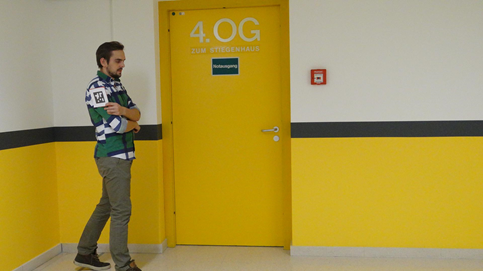
\includegraphics{testimg1.png}
	\label{fig1}
\end{figure}
\begin{figure}[ht]
	\centering
	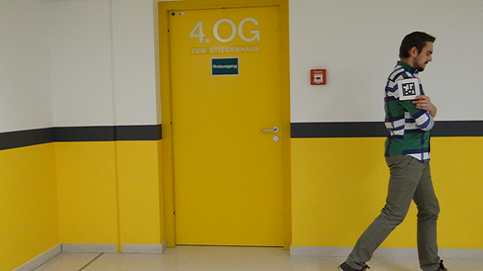
\includegraphics{testimg2.png}
	\caption{Gültiger Input}
	\label{fig2}
\end{figure}
Anhand des Markers wird das Verhältnis von einem Pixel zu einem Zentimeter festgelegt.
Dieser ist nicht in beiden Bild zwingend notwendig, muss aber vorher eingelesen werden um ihn im Datensatz selbst wiederfinden zu können. In diesem Fall hat das schwarze Quadrat eine Seitenlänge von 8cm.
Da beide Hintergründe gleich sind, werden die zwei Bilder subtrahiert und man erhält zwei mal die Person auf einem Bild (alte und neue Position). Nun kann die zurückgelegte Distanz ermittelt und anhand der Zeitangabe die Geschwindigkeit errechnet werden.

Ungültiger Input

\begin{figure}[ht]
	\centering
	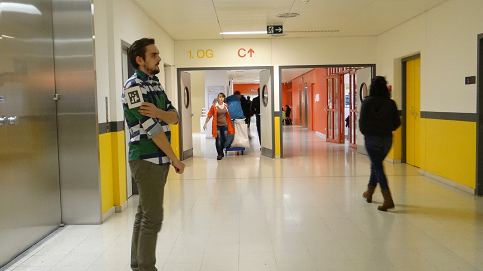
\includegraphics{ungueltig1.png}
	\label{fig3}
\end{figure}
\begin{figure}[ht]
	\centering
	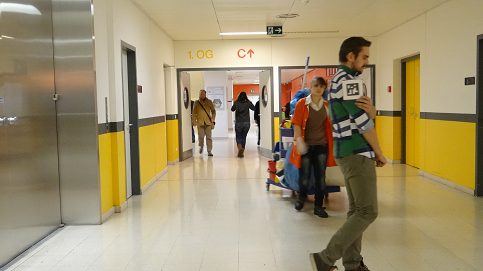
\includegraphics{ungueltig2.png}
	\caption{Ungültiger Input}
	\label{fig4}
\end{figure}
Beim Subtrahieren der beiden Bilder, werden zu viele Merkmale übrig bleiben was die Distanzberechnung wesentlich erschweren würde.

Ungültiger Input mit motion blur

\begin{figure}[ht]
	\centering
	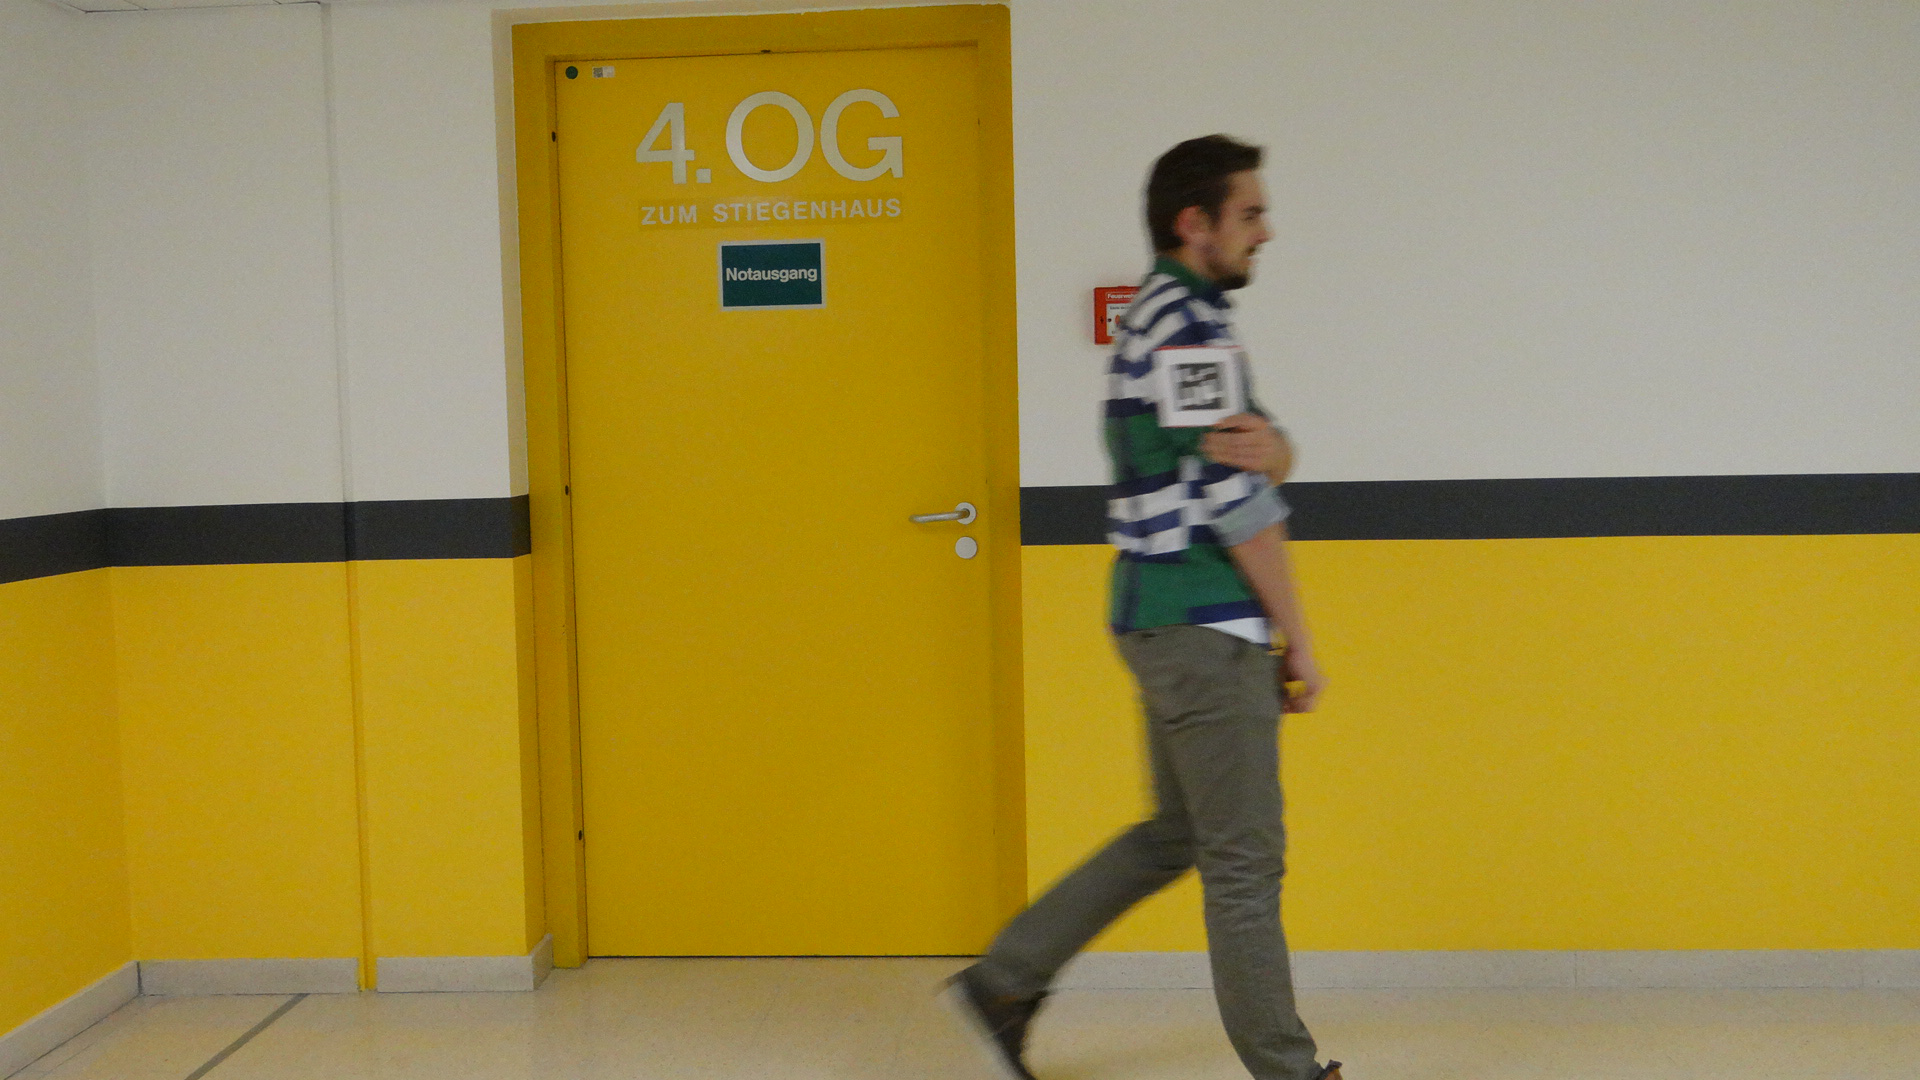
\includegraphics{ungueltig3.png}
	\label{fig5}
\end{figure}
In diesem Beispiel wird es schwer den Marker zu finden und das Pixel-Zentimeter Verhältnis zu ungenau.

\section{Zeitplan}

\begin{center}
	\begin{table}
		\begin{tabularx}{\textwidth}{ |X|X|X| }
			\hline
			Meilenstein & abgeschlossen am & Arbeitsaufwand in Stunden\\
			\hline		
			Marker im Originalbild erkennen & 11.11.2015 &	50 \\
			\hline
			Geschwindigkeit mit Matlab funktionen berechnen & 25.11.2015 & 50\\ 
			\hline
			Testdurchläufe durchführen & 1.1.2016 & 20 \\
			\hline
			CCL ausprogrammieren & 7.1.2016 & 30\\
			\hline		
			Morphologische Operationen ausprogrammieren & 15.12 & 30 \\
			\hline
			Threshold by Otsu ausprogrammieren & 10.12 & 20 \\
			\hline
			Evaluation & 20.12.2016 & 20 \\
			\hline
			Documentation & 7.1.2016 & 30 \\
			\hline
			\hline
			Summe & 7.1.2016 & 250 \\
			\hline
		\end{tabularx}	
		\caption{Unser endgültiger Zeitplan}
		\label{table:zeitplan}
	\end{table}
\end{center}

%%------------------------------------------------------

%%------------------------------------------------------
\section{Arbeitsteilung}

\begin{center}
	\begin{table}
	\begin{tabularx} {\textwidth}{ |X | X | }
		\hline
		Name & Tätigkeiten\\
		\hline
		Thomas Pinetz & CCL Implementierung, Threshold von Otsu, \newline Pixeldistanz Prototyp, Bericht Sektion Methodik \\
		\hline
		Andreas Seiwaldstätter & MyGetBiggestComponents/MyAreaOpen Implementierung, \newline Bericht Sektion Evaluierung...\\
		\hline
		\hline
		Elvis Dzafic & RANSAC Implementierung,Erosion und Dilation Implementierung \newline Bericht Sektion Implementierung..\\
		\hline
		\hline
		Vorname2 Nachname2 & Matlab-Funktion C, Bericht Abschnitt D...\\
		\hline
	\end{tabularx}
		\caption{Unsere Arbeitsteilung}
		\label{table:arbeitsteilung}	
	\end{table}
\end{center}

%%------------------------------------------------------

%%------------------------------------------------------
\section{Methodik}

Unser Workflow setzt sich wie folgt zusammen. Zuerst muss die Distanz zur Kamera erkannt werden. Dafür brauchen wir einen Marker, von welchem wir die tatsächliche Größe in der realen Welt kennen. Dann muss ein Foto von der richtigen Distanz gemacht werden. Dadurch können wir von der Größe des Markers auf die Größe der Objekte schließen. 

Danach brauchen wir 2 Bilder von einem Objekt mit statischen Hintergrund um die Geschwindigkeits- beziehungsweise Distanzmessung zu vollziehen, wobei eins der Bilder auch den Marker enthalten kann um die zuvor erwähnte Distanzmessung zu vollziehen.

Diese Bilder werden mit einem Threshold zu Schwarzweißbilder verarbeitet und mit einer Kombination von Morphologischen Operationen und Connected Component Labelling ~\cite{suzuki2003linear} wird eine Bounding Box um die 2 Objekte gelegt um den Mittelpunkt zu berechnen und danach die Distanz auszurechnen.

Der Marker wird von uns mittels \textbf{Speeded up robust features (SURF)} ~\cite{bay2006surf} gefunden. Wir haben an dieser Stelle auch andere Möglichkeiten probiert. In die engere Auswahl sind auch \textbf{Scale Invariant Feature Transform} ~\cite{lowe2004distinctive} und \textbf{Oriented FAST and Rotated BRIEF (ORB)} ~\cite{rublee2011orb}. Auf Grund des nativen Supports und da wir die Methode nicht selbst implementiert haben, haben wir uns dann für SURF entschieden. 

Auf Grund der gefundenen Keypoints wird dann dann die Bounding Box mittels \textbf{random sample consensus (RANSAC)} ~\cite{fischler1981random} erstellt. Die Pixelgröße dieser Bounding Box wird dann benutzt um von der bekannten Größe des Markers auf die Pixeldistanz umzurechnen.

Auch für die Pixeldistanzberechnung der beiden Objekten aus den Bildern haben wir verschiedene Ansätze. Jeder unserer Ansätze beginnt damit, dass wir die Bilder voneinander abziehen und dann über einen Thresholdingalgorithmus ein Schwarzweisbild zu erstellen. Dabei haben wir das Problem, dass man den Schwellwert richtig bestimmen muss. Dafür haben wir den Threshold von Otsu implementiert ~\cite{otsu1975threshold}. In unserem Ansatz haben wir dann eine Kombination aus Morphologischen Operationen und Connected Component Labeling genommen um die 2 Regionen zu finden, welche zu den zwei Objekten gehören. Dieser Ansatz hat den Vorteil, dass auch wenn sich der Hintergrund ein bisschen ändert kann man mit den Morphologischen Operation darauf reagieren. Daher, wenn das Connected Component Labeling mehr als 2 Components erkennt, kann man Erosion anwenden um zusätzliche Components zu ignorieren. Auch kann man damit relativ gut beide Objekte voneinander trennen. Für diesen Zweck haben wir ein Connected Component Labeling und die Morphologischen Operationen implementiert.

Ein anderer Ansatz war bei der Mitte aller Punkte eine vertikale Linie durchzulegen und dann aus den resultierenden zwei Bildern den Mittelpunkt der Objekte zu berechnen. Das Problem dabei, war dass die Objekte eventuell nicht mit einer vertikalen linie getrennt werden können. Auch verändert jede Änderung im Hintergrund den Mittelwert und verfälscht dadurch die Messung. Auch kann es zu Veränderungem im zum messenden Objekt kommen. Zum Beispiel können die Hände bei einem Menschen einmal ausgestreckt sein und ein anderes mal nicht. Dadurch würde sich der Mittelwert verändern und auch die Segmentierung kann dadurch falsch werden.

Nachdem man die beiden Mittelpunkte gefunden hat kann man sich mit trivialer Geometrie die euklidische Pixeldistanz ausrechnen und mit dem Faktor multiplizieren, welchen man im Ersten Schritt ausgerechnet hat. Dividiert durch die Zeit ergibt dann die Durchschnittsgeschwindigkeit.


\section{Implementierung}
(1-X Seiten)\\
Hier gebt ihr einen Überblick über eure Implementierung:\\
Wie habt ihr die im vorhergehenden Abschnitt vorgestellte Methodik praktisch umgesetzt? Wie werden die einzelnen Methoden kombiniert (zB. Implementierungspipeline)?\\
Hier ist Platz für Implementierungsdetails wie zB. gewählte Parameter. \\
Wie startet der User das Programm? Welche Parameter hat der User zu setzen?\\
Auch in diesem Abschnitt können Referenzen und Zitate notwendig sein.\\

Hier gebt ihr einen Überblick über eure Implementierung:\\
Wie habt ihr die im vorhergehenden Abschnitt vorgestellte Methodik praktisch umgesetzt? Wie werden die einzelnen Methoden kombiniert (zB. Implementierungspipeline)?
Hier ist Platz für Implementierungsdetails wie zB. gewählte Parameter.
Wie startet der User das Programm? Welche Parameter hat der User zu setzen?
Auch in diesem Abschnitt können Referenzen und Zitate notwendig sein.\\

Die erste Hürde war die sinnvolle und gleichmäßige Arbeitsaufteilung. Gruppen-intern wurde die Methodik Figure \ref{fig:implPipeline}

\begin{figure}[h]
\centering
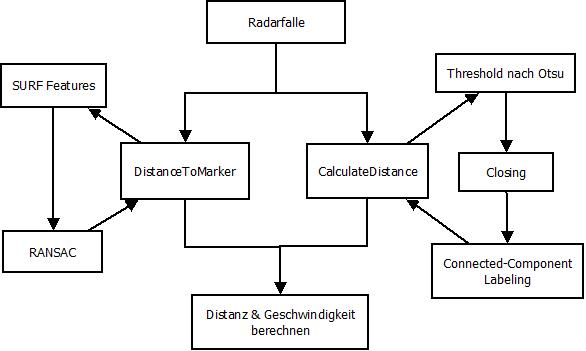
\includegraphics[scale=0.8]{Implementationspipeline}
\caption{Implementierungs-Pipeline}
\label{fig:implPipeline}
\end{figure}

%%------------------------------------------------------

%%------------------------------------------------------
\section{Evaluierung}
Unser Datensatz setzt sich sowohl aus Testbildern zusammen, für die unsere Radarfalle funktioniert, als auch aus solchen, bei denen dies nicht der Fall ist. Sämtliche Bilder (bis auf wenige Ausnahmen), die sich im Datensatz befinden, wurden selbst geschossen, mit einer SONY Kamera, Modell DSC-HX200V, auf einem Stativ. Das Benützen eines Stativs ist wichtig, um Verwackelungen, die eine falsche Identifizierung des bewegten Objektes zur Folge haben, zu vermeiden. Als Argument für strel (3. Argument von radarFalle) wurde jedes mal 'square' verwendet.

Der erste Datensatz, für den die Radarfalle auch funktioniert, setzt sich aus folgenden Bildern zusammen: 
\begin{itemize}
	\item ../Assets/Marker/i1.jpg für den Marker (die reelle Größe dieses Markers ist die eines A4 Blattes, also sqrt(210$^2$ + 297$^2$)), 
	\item ../Assets/x1.jpg als Bild in dem der Marker gesucht wird
	\item ../Assets/x2.jpg und ../Assets/x3.jpg als Bilder, in denen die Distanz gemessen wird
\end{itemize}
Für diesen Datensatz wird die richtige Distanz von 2,25m berechnet (und daher auch die richtige Geschwindigkeit). Zum Vergleich: Eine Fliese hat ca. 30cm Breite und ca. 7,5 Fliesen befinden sich zwischen Anfangs- und Endposition. Die Größe der Bilder ist 2mp, was ausreichend ist, um den Marker zu erkennen, jedoch noch nicht so groß ist, dass das Programm zu lange für die Berechnung braucht (Vgl. Datensatz2).

Der zweite Datensatz, für den die Radarfalle ein richtiges Ergebnis zurückliefert, ist flogender:
\begin{itemize}
	\item ../Assets/Marker/i1.jpg für den Marker (die reelle Größe dieses Markers ist die eines A4 Blattes, also sqrt(210$^2$ + 297$^2$)), 
	\item ../Assets/f1.jpg bzw. ..Assets/f1b.jpg als Bild in dem der Marker gesucht wird
	\item ../Assets/f2.jpg und ../Assets/f3.jpg als Bilder, in denen die Distanz gemessen wird
\end{itemize}
Der errechnete, zurückgelieferte Wert entspricht einer Distanz von 1,25m was der tatsächlichen Distanz erneut sehr nahe kommt (Vergleich: etwas mehr als 4 Fliesen á 30cm liegen zwischen Anfangs- und Endposition). Die Bilder haben eine Größe von 5mp, was, im Vergleich zu Datensatz1, zu einer merkbar längeren Berechnungszeit führt. Es wird auch ein korrektes Ergebnis zurückgeliefert, wählt man f1b.jpg als Bild in dem der Marker gesucht wird, wobei kleinere Schwankungen des Ergebnisses immer möglich sind, da der verwendete RANSAC Algorithmus zur Berechnung der Bounding Box des Markers eine Funktion ist, die mit zufälligen Werten arbeitet.

Der folgende Datensatz funktioniert zwar, benötigt jedoch viel Zeit zur Berechnung, da die Eingabebilder eine Größe von 8mp haben. Wir empfehlen daher nur Bilder der Größe 2mp zu verwenden:
\begin{itemize}
	\item ../Assets/Marker/Marker.png für den Marker (die reelle Größe dieses Markers ist 80x80mm, also sqrt(80$^2$ + 80$^2$)), 
	\item ../Assets/move2.jpg als Bild in dem der Marker gesucht wird
	\item ../Assets/move1.jpg und ../Assets/move2.jpg als Bilder, in denen die Distanz gemessen wird
\end{itemize}
Das zurückgelieferte Ergebnis ist 1,42m, was der tatsächlichen Distanz sehr nahe kommt (etwas weniger als 5 Fliesen).

Der folgende Datensatz funktioniert nicht, da der Marker nicht gefunden werden kann (weil er keinen weißen Hintergrund hat):
\begin{itemize}
	\item ../Assets/Marker/Marker.png für den Marker (die reelle Größe dieses Markers ist 80x80mm, also sqrt(80$^2$ + 80$^2$)), 
	\item ../Assets/2mpNoStativ1.jpg als Bild in dem der Marker gesucht wird
	\item ../Assets/2mpNoStativ1.jpg und ../Assets/2mpNoStativ2.jpg als Bilder, in denen die Distanz gemessen wird
\end{itemize}
Das zurückgelieferte Ergebnis ist Inf, sowohl bei der Distanz, als auch bei der Geschwindigkeit, da die Größe in Pixel des Markers in 2mpNoStativ nicht ermittelt werden konnte. Dieser Datensatz soll illustrieren, wie wichtig es ist, den Marker deutlich und für das Programm auffindbar im Bild zu platzieren. Erreicht wird dies, indem der gewählte Marker eine Struktur hat, die nicht im Bild vorkommt, und sich deutlich vom Hintergrund abhebt.
Dieser Datensatz ist die oben bereits erwähnte Ausnahme, die nicht mit der SONY Kamera geschossen wurde, sondern mit einem iPhone 4S.

Zu den Evaluierungsfragen:

%%------------------------------------------------------
\begin{itemize}
	\item Für welche Bilder kann ein korrektes Ergebnis erzielt werden? 
	
	Die beiden Eingangsbilder dürfen sich im Hintergrund nicht unterscheiden, und nur das Objekt, dessen zurückgelegte Distanz/Geschwindigkeit ermittelt werden soll darf sich bewegt haben. Weiters muss das Objekt sich über eine Distanz bewegt haben, sodass es sich, wenn man die beiden Bilder übereinander legt, in keinem Punkt berührt. Ansonsten kann es zu einer falschen Distanzberechnung kommen, da nicht die richtigen Objekte überprüft werden. Geprüft werden können die Objekte im sich öffnenden Fenster 'After Closing'.
	\item Wird der Marker gefunden? 
	
	Der Marker muss in einem der beiden Eingangsbilder auffindbar sein. Liefert das Programm 'Inf' für Distanz und Geschwindigkeit, so ist zu überprüfen ob der (richtige) Marker gefunden wurde (im geöffneten Fenster 'Putatively Matched Points') und ob die Bounding Box richtig ermittelt wurde (im geöffneten Fenster 'Detected Box' ). Ist dies nicht der Fall, so ist möglicherweise ein besserer Marker zu wählen, oder ein schärferes Bild zu schießen.
	\item Um wie viel weicht das Ergebnis vom korrekten Wert ab? 
	
	Die Abweichung lässt sich ermitteln, indem man die Differenz der gemessenen Distanz und die der errechneten ermitelt. Die von uns ermittelte Abweichung beträgt höchstens 10\% der gesamten ermittelten Distanz (siehe oben: Vorstellung der Datensätze und errechnete Distanzen).
\end{itemize}

%%------------------------------------------------------

%%------------------------------------------------------
\section{Schlusswort}
Zusammenfassend ist zu sagen, dass wir in mehr Probleme geraten sind als erwartet. Zuerst hat uns die Markerdetektion Probleme bereitet, da wir einen Marker verwendet haben, der nicht genug markante Punkte besessen hat. Dann hatten wir Probleme mit der Auflösung, da wir nicht genügend gute Punkte finden konnten und das hat sich durch die gesamte Gruppenarbeit so weiter gezogen. Hier eine Liste der immer noch offenen Probleme:    

\begin{description}
	\item[Offene Probleme] ~\par
	\begin{itemize}
		\item Zeitliche Genauigkeit: Leider haben wir bei unseren Bildern die Zeit nur auf Sekundengenauigkeit auslesen können. Für die Radarfalle wären aber auch die Millisekunden entscheidend gewesen. Leider haben wir keine Lösung für dieses Problem gefunden, als die Zeit zwischen dem Abdrücken der Fotos manuell einzugeben oder vorher schon festzulegen.
		\item RANSAC Genauigkeit: Wenn nicht genügend gute SURF features gefunden, kann RANSAC die Box entweder nicht oder nur sehr schlecht zeichnen. Dadurch wird die Geschwindigkeit natürlich stark beeinträchtigt. Auch wenn hinreichend gute SURF features gefunden werden, können die geometrischen Elemente meist nicht zu $100\%$ beschrieben werden. Daher wird die Box leider nicht genau gezeichnet. Dadurch ist der Marker im Bild größer als er eigentlich sein sollte und die Distanz- beziehungsweise Geschwindigkeitsberechnung wird dadurch leicht verzerrt.
	\end{itemize}
\end{description}

Wir waren daher eher überrascht, dass die Methoden nicht so gut funktioniert haben wie zu Beginn der Lehrveranstaltung erhofft. Dennoch hat es uns viel Spaß gemacht die Parameter zu verändern und dann zu schauen wie sich dass auf die Zusammenhänge im Programm auswirkt.  

%%------------------------------------------------------


\bibliographystyle{plain}
\nocite{*}
\bibliography{edvb_lit}
%%Bei verwendung von Latex schreibt ihr eure Referenzen in ein eigenes bib-File (siehe hier Beispiel in edbv_lit.bib). Weitere Information zum Einbinden von BibTex gibt es hier: http://www.bibtex.org/Using/de/
%%------------------------------------------------------

\end{document}
